
%--------------------------------------------------------------------------------------
% Alapbeállítások
%--------------------------------------------------------------------------------------
\documentclass[12pt,a4paper,oneside]{report}
\usepackage[magyar]{babel} % Language support
\usepackage{geometry}
\usepackage{amsfonts,amsmath,amssymb} % Mathematical symbols
\usepackage{microtype} % Imrovements to typesetting
\usepackage{setspace} % For setting line spacing
\usepackage{cmap} % Enables more advenced text copying from the PDF document
\usepackage{sectsty} % Section heading styling

\usepackage{todonotes}

%\usepackage[backend=biber, sorting=none]{biblatex} % sorting=none a hivatkozások sorrendjéhez
%\addbibresource{mybib.bib} % A BibTeX adatbázisfájlod

\usepackage[unicode]{hyperref} % For hyperlinks in the generated document
\usepackage{booktabs} % For publication quality tables for LaTeX
\usepackage{graphicx} % For figure sizing
\usepackage{wrapfig}
\usepackage{float}
\usepackage[hang]{caption}
\usepackage{xcolor} % For code coloring in listings
\usepackage{listings} % For source code snippets
\usepackage[amsmath,thmmarks]{ntheorem} % Theorem-like environments

\usepackage[numbers]{natbib} % Bibliography

%\usepackage[T1]{fontenc} %Betűtípus beállításhoz

\usepackage{fontspec}
\setmainfont{Liberation Serif}
\usepackage{lipsum}
\usepackage{tikz}
\usepackage{pdfpages}
%\usepackage{floatrow}

\newcommand{\tss}{\textsuperscript}     % tss = felső index


%--------------------------------------------------------------------------------------
% Elnevezések
%--------------------------------------------------------------------------------------
\newcommand{\elte}{Eötvös Loránd Tudományegyetem}
\newcommand{\ik}{Informatikai Kar}
\newcommand{\smi}{Savaria Műszaki Intézet}

\newcommand{\keszitette}{Horváth Milán}\newcommand{\konzulens}{Konzulens}
\newcommand{\temavezeto}{Témavezető}
\newcommand{\selectbsc}{
  \newcommand{\munkatipus}{Diplomamunka}       % Dokumentum típusa
  \newcommand{\munkatipusHU}{Diplomamunka}     % Dokumentum típusa
  \newcommand{\munkatipusok}{Diplomamunkák}   % többesszámban
  \newcommand{\munkatipustHU}{Diplomamunkát}  % tárgyraggal
}
\newcommand{\pelda}{Példa}
\newcommand{\definicio}{Definíció}
\newcommand{\tetel}{Tétel}
\newcommand{\jelolesek}{Jelölések jegyzéke}
\newcommand{\eloszo}{Előszó}
\newcommand{\bevezetes}{Bevezetés}
\newcommand{\koszonetnyilvanitas}{Köszönetnyilvánítás}
\newcommand{\osszefoglalas}{Összefoglalás}
\newcommand{\summary}{Summary}
\newcommand{\fuggelek}{Függelék}
\newcommand{\melleklet}{Mellékletek}
\newcommand{\authorName}{\authorFamilyName{} \authorGivenName}
\newcommand{\consulentA}{\consulentATitle\consulentAFamilyName{} \consulentAGivenName}
\newcommand{\consulentB}{\consulentBTitle\consulentBFamilyName{} \consulentBGivenName}
\newcommand{\consulentC}{\consulentCTitle\consulentCFamilyName{} \consulentCGivenName}
\newcommand{\supervisor}{\supervisorTitle\supervisorFamilyName{}
\supervisorGivenName}

\newcommand{\selectthesislanguage}{\selecthungarian}
\newcommand{\selectforeignlanguage}{\selectenglish}


\def\lstlistingname{lista}

\newcommand{\appendixletter}{6} % a fofejezet-szamlalo az angol ABC 6. betuje (F) lesz
\newcommand{\annexletter}{13} % M betű

%--------------------------------------------------------------------------------------
% Oldal elrendezés
%--------------------------------------------------------------------------------------
\pagestyle{plain}
\geometry{inner=35mm, outer=25mm, top=25mm, bottom=25mm}

%--------------------------------------------------------------------------------------
% Szöveg és bekezdés stílus
%--------------------------------------------------------------------------------------
\sectionfont{\Large\upshape\bfseries}  % Section title font
\subsectionfont{\Large\itshape\mdseries}
\subsubsectionfont{\large\itshape\mdseries}
\setcounter{secnumdepth}{3}             % Section numbering depth

\sloppy                                 % Prevent text from spilling over the margin
\widowpenalty=10000 \clubpenalty=10000  % Prevent widow and oprhan rows
\def\hyph{-\penalty0\hskip0pt\relax}    % Enable hyphenation

\onehalfspacing                         % 1.5x Line spacing

\newcommand{\selecthungarian}{
	\selectlanguage{magyar}
	\setlength{\parindent}{2em}			% Paragraph indentation
	\setlength{\parskip}{5pt}			% Paragraph spacing
	\frenchspacing
}

%--------------------------------------------------------------------------------------
% hyperref package beállítás
%--------------------------------------------------------------------------------------
\hypersetup{
    % bookmarks=true,            % show bookmarks bar?
    unicode=true,                % non-Latin characters in Acrobat's bookmarks
    pdfnewwindow=true,           % links in new window
    colorlinks=true,             % false: boxed links; true: colored links
    linkcolor=black,             % color of internal links
    citecolor=black,             % color of links to bibliography
    filecolor=black,             % color of file links
    urlcolor=black               % color of external links
}

%--------------------------------------------------------------------------------------
% Apply variables
%--------------------------------------------------------------------------------------
% This command is called in the main tex file and uses variables set there.
\newcommand{\applyvariables}{
	\author{\authorName}
	\title{\thesisTitle}

	\hypersetup{
		pdftitle={\thesisTitle},     % title
		pdfauthor={\authorName},     % author
		pdfsubject={\munkatipus}, % subject of the document
		pdfkeywords={\keywords},     % list of keywords (separate then by comma)
		pdfproducer={\authorName},   % producer of the document (organization)
		pdfcreator={LaTeX}           % creator of the document (application)
	}
}

%--------------------------------------------------------------------------------------
% Set up listings
%--------------------------------------------------------------------------------------
\definecolor{lightgray}{rgb}{0.95,0.95,0.95}
\lstset{
	basicstyle=\scriptsize\ttfamily, % print whole listing small
	keywordstyle=\color{black}\bfseries, % bold black keywords
	identifierstyle=, % nothing happens
	% default behavior: comments in italic, to change use
	% commentstyle=\color{green}, % for e.g. green comments
	stringstyle=\scriptsize,
	showstringspaces=false, % no special string spaces
	aboveskip=3pt,
	belowskip=3pt,
	backgroundcolor=\color{lightgray},
	columns=flexible,
	keepspaces=true,
	escapeinside={(*@}{@*)},
	captionpos=b,
	breaklines=true,
	frame=single,
	float=!ht,
	tabsize=2,
	literate=*
		{á}{{\'a}}1	{é}{{\'e}}1	{í}{{\'i}}1	{ó}{{\'o}}1	{ö}{{\"o}}1	{ő}{{\H{o}}}1	{ú}{{\'u}}1	{ü}{{\"u}}1	{ű}{{\H{u}}}1
		{Á}{{\'A}}1	{É}{{\'E}}1	{Í}{{\'I}}1	{Ó}{{\'O}}1	{Ö}{{\"O}}1	{Ő}{{\H{O}}}1	{Ú}{{\'U}}1	{Ü}{{\"U}}1	{Ű}{{\H{U}}}1
}

%--------------------------------------------------------------------------------------
% Setup captions
%--------------------------------------------------------------------------------------
\captionsetup[figure]{
	width=.75\textwidth,
	aboveskip=10pt}

\renewcommand{\captionlabelfont}{\it}
\renewcommand{\captionfont}{\footnotesize\it}



%%%%%%%%%%%%%%%%%%%%%%%%%%%%%%%%%%%%%%%%%%%%%%%%%%%%%%%%%%%%%%%%%%%%%%%%%%%%%%%%%%
%%%%%%%%%%%%%%%%%%%%%%%%%%%%%%%%%%%%%%%%%%%%%%%%%%%%%%%%%%%%%%%%%%%%%%%%%%%%%%%%%%
%%%%%%%%%%%%%%%%%%%%%%%%%%%%%%%%%%%%%%%%%%%%%%%%%%%%%%%%%%%%%%%%%%%%%%%%%%%%%%%%%%



\selectbsc
%--------------------------------------------------------------------------------------
% Változók beállítása [Setting variables]
%--------------------------------------------------------------------------------------
%TODO Állítsd be az alábbi változókat [Set these variables]%
% Szerző [Author]
\def\authorFamilyName{Horváth}
\def\authorGivenName{Milán}
\def\neptun{MYQGQ0}

% Konzulens 1 [Consulent 1]
\def\consulentATitle{}
\def\consulentAFamilyName{Bátorfi}
\def\consulentAGivenName{János György}
\def\consulentARank{egyetemi tanársegéd}

% Konzulens 2 [Consulent 2], ha nincs hagyd üresen
\def\consulentBTitle{}
\def\consulentBFamilyName{}
\def\consulentBGivenName{}
\def\consulentBRank{}

% Konzulens 3 [Consulent 3], ha nincs hagyd üresen
\def\consulentCTitle{}
\def\consulentCFamilyName{}
\def\consulentCGivenName{}
\def\consulentCRank{}

% Témavezető
\def\supervisorTitle{Prof. Dr.}
\def\supervisorFamilyName{Sidor}
\def\supervisorGivenName{Jurij}
\def\supervisorRank{egyetemi tanár}

% Dolgozat címe [Thesis title]
\def\thesisTitle{Diplomamunka}

% Kulcsszavak (a PDF-be) [Keywords (to PDF)]
\def\keywords{mechatronika, szabályozástechnika, etorobotika, ipar 4.0}

% Tanszék [Department]
\def\department{\smi}

% Elzártan kezelendő dolgozat [Restricted access]
%TODO Töltsd ki a korlátozás lejártának dátumát!
\def\endOfRestrictedAccess{2034 január 31. nap}

% Változók beállítása a PDF fájlhoz [Apply variables for the PDF file]
\applyvariables



%%%%%%%%%%%%%%%%%%%%%%%%%%%%%%%%%%%%%%%%%%%%%%%%%%%%%%%%%%%%%%%%%%%%%%%%%%%%%%%%%%
%%%%%%%%%%%%%%%%%%%%%%%%%%%%%%%%%%%%%%%%%%%%%%%%%%%%%%%%%%%%%%%%%%%%%%%%%%%%%%%%%%
%%%%%%%%%%%%%%%%%%%%%%%%%%%%%%%%%%%%%%%%%%%%%%%%%%%%%%%%%%%%%%%%%%%%%%%%%%%%%%%%%%



%--------------------------------------------------------------------------------------
% Dokumentum törzse [Document body]
%--------------------------------------------------------------------------------------
\onehalfspacing
\begin{document}

\pagenumbering{gobble}
\selectthesislanguage

% Címoldal [Titlepage]
\hypersetup{pageanchor=false}

%--------------------------------------------------------------------------------------
% Szennycímoldal [Cover title page]
%--------------------------------------------------------------------------------------

\clearpage
\begin{center}
\MakeUppercase{\authorName}\\[0.1cm]
\MakeUppercase{\munkatipus}\\[0.1cm]
\end{center}
\thispagestyle{empty}

%--------------------------------------------------------------------------------------
% Sorozatcímoldal [Series title page]
%--------------------------------------------------------------------------------------
\clearpage
\begin{center}

\MakeUppercase{\textbf{\elte}}\\[0.1cm]
\MakeUppercase{\textmd{\ik}}\\[0.1cm]
\MakeUppercase{\textmd{\department}}\\[0.8cm]
\vspace{1cm}

\includegraphics[width=40mm,keepaspectratio]{figures/elte_uj}\hspace{1cm}

\includegraphics[height=40mm,keepaspectratio]{figures/elte_ik_logo}\hspace{1cm}

\includegraphics[height=40mm,keepaspectratio]{figures/smi}\\[0.5cm]
\vspace{1cm}
\MakeUppercase{\munkatipusok}

\end{center}
\thispagestyle{empty}

%--------------------------------------------------------------------------------------
% Címoldal [Title page]
%--------------------------------------------------------------------------------------
\begin{titlepage}
\begin{center}

\MakeUppercase{\textbf{\elte}}\\[0.1cm]
\MakeUppercase{\textbf{\ik}}\\[0.1cm]
\MakeUppercase{\textbf{\department}}

\vspace{4.0cm}
{\huge \textsc{\authorName}}\\[0.8cm]
{\huge \MakeUppercase{\munkatipus}}\\[0.8cm]
{\Large \thesisTitle}

\vspace{3.0cm}

{
	\renewcommand{\arraystretch}{0.85}
	\begin{tabular}{ll}
	 \makebox[7cm][l]{\konzulens:} & \makebox[7cm][l]{\temavezeto:} \\
	 \noalign{\smallskip}
	 \makebox[7cm][l]{\hspace{1cm}\emph{\consulentA}} & \makebox[7cm][l]{\hspace{1cm}\emph{\supervisor}} \\
	 \makebox[7cm][l]{\hspace{1cm}\consulentARank} & \makebox[7cm][l]{\hspace{1cm}\supervisorRank} \\
	 \\
	 \makebox[7cm][l]{\hspace{1cm}\emph{\consulentB}} & \\
	 \makebox[7cm][l]{\hspace{1cm}\consulentBRank} & \\
	 \\
	 \makebox[7cm][l]{\hspace{1cm}\emph{\consulentC}} & \\
	 \makebox[7cm][l]{\hspace{1cm}\consulentCRank} & \\
	 
	\end{tabular}
}

\vfill
{\Large Szombathely, \the\year.}
\end{center}
\end{titlepage}
\hypersetup{pageanchor=false}
\thispagestyle{empty}
  % Diplomamunka címlap [Thesis]

% Copytightoldal [Copyright page]
%TODO Válaszd ki a megfelelőt! [Choose one]
%\selectlanguage{magyar}
\pagenumbering{gobble}
\selecthungarian
%--------------------------------------------------------------------------------------
% Copyrightoldal
%--------------------------------------------------------------------------------------
\begin{flushleft}
\szerzoijog{} {\textcopyright} \authorName, \the\year.
\end{flushleft}

\vfill
\clearpage
\thispagestyle{empty} % an empty page

\selectthesislanguage
               % Nyílt kezelésű [Open access]
\selectlanguage{magyar}
\pagenumbering{gobble}
\selecthungarian
%--------------------------------------------------------------------------------------
% Copyrightoldal
%--------------------------------------------------------------------------------------
\begin{flushleft}
Szerzői jog {\textcopyright} \authorName, \the\year.
\end{flushleft}

\vspace{0.5cm}

\begin{center}
\textbf{ZÁRADÉK}\\
\end{center}

\vspace{0.5cm}
\noindent
Ez a \MakeLowercase{\munkatipusHU} elzártan kezelendő és őrzendő, a hozzáférése a vonatkozó szabályok szerint korlátozott, a diplomamunka tartalmát csak az arra feljogosított személyek ismerhetik.

A korlátozott hozzáférés időtartamának lejártáig az arra feljogosítottakon kívül csak a korlátozást kérelmező személy vagy gazdálkodó szervezet írásos engedélyéjével rendelkező személy nyerhet betekintést a diplomamunka tartalmába.

\vspace{0.3cm}

%TODO: fill out the date
A hozzáférés korlátozása és a zárt kezelés \endOfRestrictedAccess ján ér véget.

\vspace{30pt}
\noindent Szombathely, 2024. 01. 31.
\vfill
\clearpage
\thispagestyle{empty} % an empty page

\selectthesislanguage
   % Elzárt kezelésű [Restricted access]

% Feladatkiírás [Project page]
%TODO A nyomtatott verzóban ne szerepeljen! [Remove before printing]
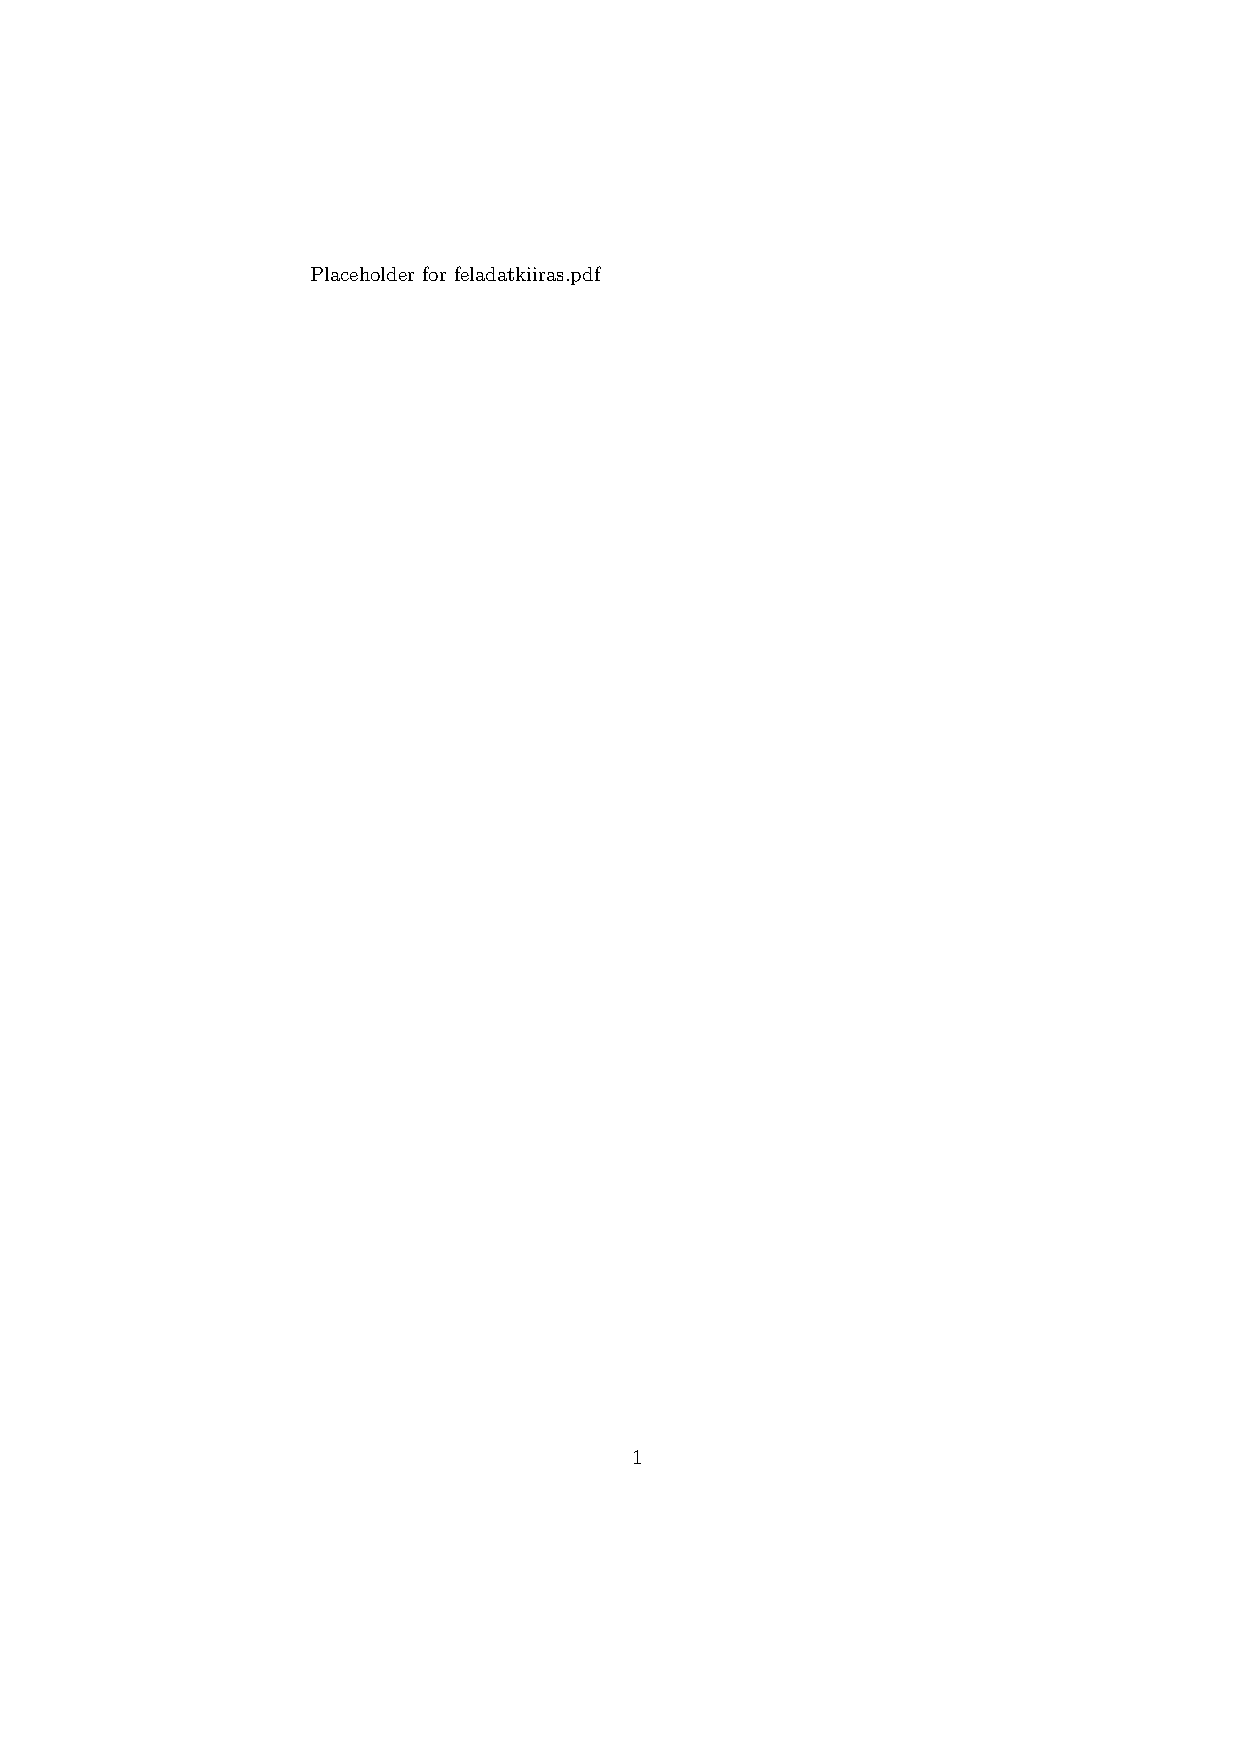
\includepdf[pages=1]{feladatkiiras.pdf}

% Nyilatkozatok [Declarations]
\selectlanguage{magyar}
\selecthungarian
\pagenumbering{roman}
\setcounter{page}{6}
\cleardoublepage % duplexnél páratlan oldalon legyen
%--------------------------------------------------------------------------------------
% Nyilatkozatok
%--------------------------------------------------------------------------------------
\begin{center}
\section*{NYILATKOZATOK}
\end{center}

\vspace{0.5cm}


%--------------------------------------------------------------------------------------

\begin{center}
\emph{Nyilatkozat az önálló munkáról}
\end{center}
Alulírott,  \emph{\authorFamilyName{} \authorGivenName} (\neptun), az Eötvös Loránd Tudományegyetem hallgatója, büntetőjogi és fegyelmi felelősségem tudatában kijelentem és sajátkezű aláírásommal igazolom, hogy ezt a \MakeLowercase{\munkatipustHU} meg nem engedett segítség nélkül, saját magam készítettem, és szakdolgozatomban csak a megadott forrásokat használtam fel. Minden olyan részt, melyet szó szerint vagy azonos értelemben, de átfogalmazva más forrásból átvettem, egyértelműen, a hatályos előírásoknak megfelelően, a forrás megadásával megjelöltem.

Ennek a szakdolgozatnak önálló, eredeti szerzője vagyok, ez az önálló szellemi alkotás jogtisztaság szempontjából megfelel az „Eötvös Loránd Tudományegyetem Szervezeti és Működési Szabályzata, II. kötet, Hallgatói Követelményrendszer. Módosításokkal egybeszerkesztett változat [2017. szeptember 1.]” c. szabályzat 74/A–74/C. §-aiban foglalt rendelkezéseknek.

\begin{flushleft}
Szombathely, \today
\end{flushleft}

\begin{flushright}
 \makebox[7cm]{\rule{6cm}{.4pt}}\\
 \makebox[7cm]{\emph{hallgató}}
\end{flushright}


\vfill
\clearpage

\selectthesislanguage

\newcounter{romanPage}
\setcounter{romanPage}{\value{page}}
\stepcounter{romanPage}


\selectthesislanguage
% Tartalomjegyzék [Table of Contents]
\setcounter{tocdepth}{3}  % Tartalomjegyzék mélysége [ToC depth]
\tableofcontents\vfill

% Ábrák és táblázatok jegyzéke [List of Figures, Tables]
%TODO Kommenteld ki, ha használni szeretnéd. [Uncomment to use]
%\listoffigures\addcontentsline{toc}{chapter}{\listfigurename}   % Ábrák jegyzéke - opcionális
%\listoftables\addcontentsline{toc}{chapter}{\listtablename}     % Táblázatok jegyzéke - opcionális

\chapter*{Előszó}\addcontentsline{toc}{chapter}{\eloszo}
Már a középiskolás éveim során érdeklődtem a 3D tervezés, a CAD-CAM világa felé. Gépi forgácsoló szakmámból kifolyólag elég régóta kürölvesz engem a gépészeti világ és akkor jött a gondolat, mi lenne ha jelentkeznék egyetemre. Életem egyik legjobb döntése volt a gépészmérnöki képzés elkezdése. Rengeteg új információval gazdagodtam, sokkal jobban el tudtam mélyülni a CAD-CAM rendszerekben, valamint megismerkedtem számomra addig teljesen ismeretlen módszerekkel. Az egyik ilyen volt a végeselem analízis. Ez a terület tetszett meg a legjobban a képzés során, rengeteg lehetőség rejlik benne. A diplomamunka téma kiválasztásánál számomra fontos volt, hogy a CAD-CAM, valamint a végeselem analízis szerepet kapjanak az elkészítés során.


\begin{center}
    $\thicksim \; \thicksim \; \thicksim$
\end{center}


\subsubsection*{Köszönetnyilvánítás}
\emph{Ha kell}

\vspace{0.5cm}

\begin{flushleft}
{Szombathely, \today}
\end{flushleft}

\begin{flushright}
\emph{\authorName}
\end{flushright}
\vfill

\chapter*{Jelölések}\addcontentsline{toc}{chapter}{\jelolesek}
%----------------------------------------------------------------------------

A táblázatban a többször előforduló jelölések magyar és angol nyelvű elnevezése,
valamint a fizikai mennyiségek esetén annak mértékegysége található. Az egyes
mennyiségek jelölése – ahol lehetséges – megegyezik hazai és a nemzetközi
szakirodalomban elfogadott jelölésekkel. A ritkán alkalmazott jelölések
magyarázata első előfordulási helyüknél található.

%~~~~~~~~~~~~~~~~~~~~~~~~~~~~~~~~~~~~~~~~~~~~~~~~~~~~~~~~~~~~~~~~~~~~~~~~~~~~~~~~~~~~~
% A táblázatokat ABC rendben kell feltölteni, először mindig a kisbetűvel
% kezdve. Ha egyazon betűjelnek több értelmezése is van, akkor mindegyiket kü-
% lön sorban kell feltüntetni. Konstansok esetén az értéket is a táblázatba
% kell írni.
% Dimenzió nélküli mennyiségek mértékegysége 1 és nem: – !
% A jelölésjegyzékben csak SI vagy SI-n kívüli engedélyezett mértékegységeket
% szabad feltüntetni. Egy dokumentumon belül az SI és pl. az angolszász
% mértékrendszer nem keverhető!
%~~~~~~~~~~~~~~~~~~~~~~~~~~~~~~~~~~~~~~~~~~~~~~~~~~~~~~~~~~~~~~~~~~~~~~~~~~~~~~~~~~~~~

%~~~~~~~~~~~~~~~~~~~~~~~~~~~~~~~~~~~~~~~~~~~~~~~~~~~~~~~~~~~~~~~~~~~~~~~~~~~~~~~~~~~~~
% A Jelölés oszlop alapvetően kurzív betűváltozattal szedendő, a Mértékegység
% oszlopot álló betűkkel kell szedni. Felső indexhez használható a \tss{}
% parancs.
%~~~~~~~~~~~~~~~~~~~~~~~~~~~~~~~~~~~~~~~~~~~~~~~~~~~~~~~~~~~~~~~~~~~~~~~~~~~~~~~~~~~~~

\def\arraystretch{1.5}%  vertical cell padding

\subsubsection*{Latin betűk}
\begin{center}
    \begin{tabular}{lp{10cm}l}
        \hline
        Jelölés & Megnevezés, megjegyzés, érték & Mértékegység \\
        \hline
        $E$     & Rugalmassági modulusz  & GPa     \\
        $F$     & erő                        & N           \\
        $S$     & keresztmetszet             & mm\tss{2} \\
        \hline
    \end{tabular}
\end{center}



\subsubsection*{Görög betűk}
\begin{center}
    \begin{tabular}{lp{10cm}l}
        \hline
        Jelölés & Megnevezés, megjegyzés, érték & Mértékegység \\
        \hline
                $\varepsilon$  & alakváltozás           & 1    \\
        $\sigma$  & feszültség                  & MPa             \\

        \hline
    \end{tabular}
\end{center}



\subsubsection*{Indexek, kitevők}
\begin{center}
    \begin{tabular}{lp{12.8cm}}
        \hline
        Jelölés & Megnevezés, értelmezés\\
        \hline
        $e$     & elem  \\
        max     & maximális érték        \\
        \hline
    \end{tabular}
\end{center}


\def\arraystretch{1}%  vertical cell padding

% Főszöveg [The main part of the thesis]
\cleardoublepage
\pagenumbering{arabic}
\chapter{Bevezetés}

A mélyhúzás a lemezalakítás egyik legösszetettebb és legszélesebb körben alkalmazott technológiája, amelynek során síklemezből háromdimenziós, üreges alkatrészeket állítanak elő. A folyamat sikerességét döntően befolyásolja a lemezanyag anizotróp viselkedése, amely a gyártási folyamat során – különösen a hengerelés következtében – kialakuló preferált kristályorientációból (textúra) ered. Az anyag irányított mechanikai tulajdonságai közvetlenül hatnak az alakíthatóságra, a fülképződésre és a végtermék minőségére.

Az anizotrópia mértékét a Lankford-paraméterrel (r-érték) jellemezzük, amely a vastagságirányú és szélességirányú alakváltozás arányát fejezi ki egytengelyű húzás során. Wu et al. (2023) kísérleti vizsgálatai rozsdamentes acél hengermélyhúzása során kimutatták, hogy az r$_{90}$ értéke 29-48\%-kal járul hozzá az aljzati visszarugózáshoz, míg az r$_{45}$ és r$_{0}$ értékek másodlagos jelentőségűek. A síkanizotrópia ($\Delta$r), amely a különböző irányokban mért r-értékek közötti eltéréseket számszerűsíti, közvetlenül felelős a fülképződés mértékéért és mintázatáért.

A képlékeny alakítás során fellépő anizotróp viselkedés pontos modellezése kritikus fontosságú a szerszámtervezésben és a folyamatoptimalizálásban. A hagyományos izotróp folyási kritériumok (von Mises, Tresca) nem képesek megfelelően leírni a lemezanyagok irányított tulajdonságait. Az elmúlt évtizedekben számos anizotróp folyási kritérium került kifejlesztésre – a klasszikus Hill'48 modellről (Hill, 1948) a fejlett Barlat-család kritériumaiig (Yld2000-2d, Yld2004-18p) –, amelyek fokozatosan javuló pontossággal írják le a valós anyagviselkedést (Chen et al., 2023).

Jelen irodalmi áttekintés célja, hogy átfogó képet nyújtson a mélyhúzás folyamatáról, a lemezanyagok anizotróp viselkedésének fizikai hátteréről, a szerszámtervezés alapelveiről, valamint a modern végeselem-módszer (VEM) alkalmazásáról. Külön hangsúlyt helyezünk az anyagfüggő viselkedésre és a kristályszerkezet szerepére, mivel ezek az alapvető tényezők határozzák meg a mélyhúzhatóságot és az ipari folyamatok megbízhatóságát.

\chapter{Irodalmi áttekintés}

\section{Képlékeny alakítás elméleti alapjai}
\subsection{Rugalmas és képlékeny alakváltozás}

A képlékeny alakítás olyan technológiai folyamatok összessége, amelyek során a fém vagy ötvözet munkadarabot külső mechanikai erőhatással, maradandó (képlékeny) alakváltozás révén alakítjuk át kívánt formára, miközben az anyag térfogata és tömege változatlan marad \cite{Gillemot1977}. A folyamat alapja az anyag képlékeny viselkedése: a ráhatáskor fellépő feszültség túllépi a folyáshatárt, így az anyag a tehermentesítést követően sem tér vissza eredeti alakjára.

Az alakítási folyamatok a hőmérséklettől függően két alapvető csoportra oszthatók, amelyek különböző mikroszerkezeti folyamatokat és technológiai jellemzőket eredményeznek.

\subsubsection*{Hidegalakítás}
Hidegalakítás ($T < 0,3T_m$, ahol $T_m$ az olvadáspont Kelvinben): A szobahőmérsékleten vagy közel ahhoz végzett alakítás során az anyag képlékenyen deformálódik, de az alakváltozás mechanizmusai (diszlokációs mozgás, csúszás) nem járnak újrakristályosodással. A hidegalakítás jellemzői:
\begin{itemize}
    \item Kiváló méretpontosság (IT12-IT14 tolerancia)
    \item Jó felületi minőség
    \item Növekedő szilárdság és keménység (alakítási keményedés)
    \item Csökkenő képlékenység
    \item Textúra kialakulása és stabilizálódása
    \item Maradó feszültségek jelenléte
\end{itemize}
Acéllemezeknél a szobahőmérsékletű alakítás uralkodó a járműipari alkalmazásokban, ahol a dimenzionális stabilitás és a felületi minőség kritikus követelmény. Az alumíniumötvözetek szintén kiválóan hidegalakíthatók az FCC kristályszerkezetből adódó jó szobahőmérsékletű képlékenységük miatt.

\subsubsection*{Melegalakítás}
Melegalakítás ($T > 0,5-0,6T_m$): Magasabb hőmérsékleten végzett alakítás során a képlékeny deformáció egyidejűleg zajlik a dinamikus újrakristályosodással vagy dinamikus recovery folyamatokkal, ami friss, deformálatlan szemcsestruktúrát eredményez. A melegalakítás előnyei:
\begin{itemize}
    \item Jelentősen csökkentett alakítóerők
    \item Nagy alakváltozások elérhetősége egyetlen lépésben
    \item Kedvező mechanikai tulajdonságok finomabb szemcseszerkezet miatt
    \item Belső feszültségek csökkenése
    \item Nehezen alakítható anyagok megmunkálhatósága
\end{itemize}
Hátrányok közé tartozik a nagyobb energiaráfordítás, oxidációs és lekéregesedési problémák, valamint rosszabb méretpontosság és felületi minőség. A járműiparban alkalmazott korszerű nagyszilárdságú acélok (AHSS – Advanced High-Strength Steels) melegelakítása speciális keményítési eljárásokat (press hardening, hot stamping) tesz lehetővé, amelyek során a melegelakítást azonnal hűtéssel kombinálják \cite{Pereira2024}.

\subsection{Feszültség-alakváltozás kapcsolata, szakítódiagram}
Az alakíthatóság az anyag azon képessége, hogy törés nélkül mekkora mértékű képlékeny alakváltozást képes elviselni adott alakítási körülmények között. Az alakíthatóságot számos tényező befolyásolja:
\begin{itemize}
    \item \textbf{Anyagi tényezők:} Kristályszerkezet (FCC anyagok általában jobb alakíthatóságúak, mint BCC anyagok szobahőmérsékleten), kémiai összetétel és ötvözőelemek, mikroszerkezet (szemcseméret, fázisösszetétel), textúra (preferált kristályorientáció), előzetes alakváltozási történet (hideghengerlés mértéke).
    \item \textbf{Technológiai tényezők:} Alakítási hőmérséklet, alakváltozási sebesség, feszültségállapot (egytengelyű, síkbeli, háromtengelyű), súrlódási viszonyok, szerszámgeometria.
\end{itemize}
Az alakíthatóság jellemzésére több kísérleti módszer és kritérium létezik. A legismertebb az egytengelyű szakítóvizsgálatból származó szakadási nyúlás ($A_{50}$ vagy $A_{80}$), amely azonban csak közelítő képet ad a komplex alakítási folyamatok során várható viselkedésről.

Lemezalakítás esetében a Forming Limit Diagram (FLD) az iparban széles körben alkalmazott eszköz, amely a főalakváltozások síkjában ábrázolja azt a határgörbét, amely elválasztja a biztonságos alakítási tartományt a nyakképződési/szakadási zónától. Az FLD hagyományos formája Keeler és Backofen (1963) kutatásaiból származik, és számos szabványosított mérésen alapul (Nakazima-teszt, Marciniak-teszt, hidraulikus domborítási teszt) \cite{Marciniak2002}.

\cite{Takalkar2019} átfogó áttekintésükben rámutattak, hogy a hagyományos FLD nem képes előrejelezni a nyírási törésmódokat és az élrepedéseket, amelyek különösen az AHSS acélok esetében jelentenek problémát. Ennek következtében fejlettebb károsodásmodellek kerültek kifejlesztésre (MMC – Modified Mohr-Coulomb, eMMC – extended MMC, GISSMO – Generalized Incremental Stress State dependent damage MOdel), amelyek figyelembe veszik a feszültségi triaxialitást és a Lode-paraméter hatását a törési mechanizmusokra.

\section{Mikroszerkezettől a tervezésig}
Az anizotrópia azt jelenti, hogy az anyag mechanikai tulajdonságai különböző irányokban eltérők. Fémlemezeknél az anizotrópia elsődleges oka a kristályos textúra, azaz a preferált szemcseorientációk kialakulása a gyártási folyamat (hengerlés és hőkezelés) során.

\subsection{Kristályszerkezet és csúszórendszerek}
A kristályszerkezet alapvetően meghatározza a rendelkezésre álló csúszórendszerek számát és orientációját, ami döntően befolyásolja a képlékeny anizotrópiát és az alakíthatóságot.

\subsubsection*{FCC (face-centered cubic) fémek}
Az FCC szerkezetű fémek (alumínium, réz, ausztenites acél, nikkel) 12 oktaéderikus csúszórendszerrel rendelkeznek: \{111\}<110> típusú síkok és irányok. A 12 független csúszórendszer nagy szabadságot biztosít a képlékeny alakváltozáshoz, ami általában jó szobahőmérsékletű képlékenységet eredményez. Az FCC fémek gömbös illeszkedése (atomic packing factor = 0,74) és a csúszósíkok nagy sűrűsége kedvező alakíthatóságot biztosít. Az FCC anyagok hengerelése során jellemző textúrakomponensek alakulnak ki: Brass \{112\}<111>, Copper \{112\}<111>, S \{123\}<634>. Újrakristályosodás után megjelenik a Cube \{001\}<100> orientáció, amely közepes r-értékeket (r≈0,5-1,0) eredményez. \cite{Savoie1996} alumíniumlemezek vizsgálata kimutatta, hogy 20-30\% húzás után a textúra <111> és <100> szálas textúrák felé fejlődik, ami jelentősen módosítja a lokális alakíthatóságot.

\subsubsection*{BCC (body-centered cubic) fémek}
A BCC szerkezetű fémek (ferrites acél, alacsony karbontartalmú acél) elsődlegesen \{110\}<111> és \{112\}<111> rendszereken csúsznak, összesen 24-48 potenciális rendszerrel. A BCC szerkezet kisebb atomi illeszkedési faktora (0,68) és a csúszósíkok nagyobb Peierls-feszültsége miatt szobahőmérsékleten általában alacsonyabb képlékenységet mutat, mint az FCC fémek. A BCC anyagoknál az $\alpha$-szálas (\{001\}<110> → \{112\}<110>) és $\gamma$-szálas (\{111\}<110>, \{111\}<112>) textúrakomponensek kritikusak. \cite{Raabe2005} kristályplaszticitás-szimulációi bizonyították, hogy 8, 6 vagy 4 fül alakul ki a kezdeti BCC textúrától függően, és a textúra élessége közvetlenül korrelál a fülprofil élességével. A $\gamma$-szálas komponensek (\{111\}<uvw>) magas r-értékeket (r=1,5-3,0) biztosítanak, ami kiváló alakíthatóságot eredményez.

\subsection{Textúra-fejlődés az alakítás során}
A textúra nem statikus jellemző, hanem útfüggő módon fejlődik az alakítási folyamat során. \cite{Engler2025} átfogó tanulmánya szerint a textúra útfüggő módon fejlődik: a peremrégióban (síkbeli alakváltozás) P \{011\}<111> és Goss \{011\}<100> orientációk erősödnek a korai szakaszban, míg a falrégióban (egytengelyű húzás) $\alpha$D-szálas komponensek dominálnak. Ez lokális alakíthatósági különbségeket eredményez ugyanazon alkatrészen belül.

\section{Lemezek képlékeny anizotrópiája}
\subsection{Az anizotrópia}
Az anizotrópia azt jelenti, hogy az anyag mechanikai tulajdonságai különböző irányokban eltérők. Fémlemezeknél az anizotrópia elsődleges oka a kristályos textúra, azaz a preferált szemcseorientációk kialakulása a gyártási folyamat (hengerlés és hőkezelés) során. A hengerelési folyamat során nagy nyíró- és nyomó-alakváltozások érik a fémlemezt. Az egyes szemcsék nem homogén módon deformálódnak, mivel kristályorientációjuktól függően különböző csúszórendszerek aktiválódnak. A kedvezőbb orientációjú szemcsék gyorsabban alakulnak, míg mások lassabban, és ez egy preferált orientációeloszlást, azaz textúrát eredményez.

Az anizotrópia típusai:
\begin{itemize}
    \item \textbf{Normál anizotrópia (plastic strain ratio anisotropy):} Az r-érték irányfüggősége, amely a vastagságirányú alakváltozás ellenállását jellemzi. Minél nagyobb az $\bar{r}$ (átlagos r-érték), annál jobban ellenáll az anyag a vastagságcsökkenésnek, ezáltal jobb mélyhúzhatóságot mutat.
    \item \textbf{Síkbeli anizotrópia (planar anisotropy):} A különböző irányokban mért r-értékek közötti eltérés, $\Delta r = (r_0 - 2r_{45} + r_{90})/2$ képlettel számítva. Ez közvetlenül felelős a fülképződésért: $\Delta r>0$ esetén fülek alakulnak ki 0° és 90°-nál, $\Delta r<0$ esetén $\pm$45°-nál.
    \item \textbf{Folyáshatár-anizotrópia (yield strength anisotropy):} Különböző irányokban eltérő folyáshatár értékek. Ez befolyásolja az anyagáramlást és az erőeloszlást a szerszámban.
\end{itemize}

\subsection{Lankford-tényező}
A Lankford-paraméter, vagy r-érték, az anizotrópia legfontosabb mennyiségi jellemzője, amelyet William T. Lankford vezetett be 1950-ben \cite{Lankford1950}. Az r-érték az egytengelyű húzóvizsgálat során mért szélességi és vastagsági valódi képlékeny alakváltozások arányaként definiált:
$r = \varepsilon_{width} / \varepsilon_{thickness} = \ln(w/w_0) / \ln(t/t_0)$
ahol w és w₀ a pillanatnyi és kezdeti szélesség, t és t₀ a pillanatnyi és kezdeti vastagság. Az r>1 azt jelenti, hogy az anyag inkább szélességében, mint vastagságában alakul képlékenyen, ami előnyös mélyhúzásnál.
Az átlagos r-érték (normál anizotrópia): $\bar{r} = (r_0 + 2r_{45} + r_{90}) / 4$.
A síkanizotrópia (planar anisotropy): $\Delta r = (r_0 - 2r_{45} + r_{90}) / 2$.
\cite{Wu2023} kísérleti vizsgálata rozsdamentes acél hengereken kimutatta, hogy az $r_{90}$ a legnagyobb hatással van az aljzati visszarugózásra (29-48\% hozzájárulás), míg $r_{45}$ és $r_0$ másodlagos jelentőségűek.

\subsection{Csúcsosodás, az anizotrópia közvetlen hatása}
Fülképződés (earing): Az anyag síkbeli anizotrópiája ($\Delta r \neq 0$) miatt a mélyhúzott pohár szélén periodikus magasság-ingadozások alakulnak ki. A fülek száma és elhelyezkedése közvetlenül függ a kristályos textúrától:
\begin{itemize}
    \item 4 fül: Tipikus alumíniumötvözeteknél kockatextúra dominanciája esetén, 0°, 45°, 90°, 135° helyeken.
    \item 6 fül: Jellemző mélyhúzó acéloknál $\gamma$-szálas textúra esetén.
    \item 8 fül: Összetett textúra esetén, vegyes orientációs komponensekkel.
\end{itemize}
\cite{Tang2018} kereskedelmi tisztaságú titán vizsgálatakor 13,7\%-os fülmagasságot mért $\Delta r \neq 0$ esetén. A fülképződés csökkenthető optimalizált terítékalak alkalmazásával, amely figyelembe veszi az anizotróp viselkedést.

\subsection{Ideális mélyhúzható lemez}
Az optimális mélyhúzhatóság magas átlagos r-értéket ($\bar{r} \uparrow$) és a nullához közeli síkbeli anizotrópiát ($\Delta r \to 0$) igényel. A magas $\bar{r}$ érték biztosítja az elvékonyodással szembeni nagy ellenállást, míg az alacsony $\Delta r$ érték megakadályozza a fülképződést és az ezzel járó anyagveszteséget.

\section{A mélyhúzás technológiája}
\subsection{A mélyhúzás alapelvei, fázisai}
A mélyhúzás olyan lemezmegmunkálási eljárás, amelynek során síklemezt (tárcsalemezt, terítéket) bélyeg segítségével húzógyűrűn keresztül húzunk át, miközben a lemez radiális húzó- és tangenciális nyomófeszültség hatására üreges, általában forgásszimmetrikus vagy egyéb alakú alkatrésszé formálódik \cite{Gillemot1977, Weltsch2019}.
A mélyhúzás során három fő deformációs zóna különíthető el:
\begin{itemize}
    \item \textbf{Bélyeg alatti zóna (aljzat):} Itt az anyag viszonylag kis alakváltozást szenved, elsősorban hajlítási és egyenesítési cikluson megy keresztül a bélyegsugárnál.
    \item \textbf{Sugár-régiók (bélyegsugár és húzógyűrű-sugár):} Ezek a legkritikusabb zónák a legnagyobb von Mises feszültség szempontjából.
    \item \textbf{Peremzóna (flange):} A húzógyűrű és a peremtartó közötti terület, ahol az anyag radiális húzó- és tangenciális (kerületi) nyomófeszültségnek van kitéve.
\end{itemize}

\subsection{Meghatározó technológiai paraméterek}
\begin{itemize}
    \item \textbf{Határalakítási arány (LDR – Limiting Drawing Ratio):} A legnagyobb sikeresen mélyhúzható teríték átmérőjének ($D_0$) és a bélyeg átmérőjének ($d_p$) aránya: $LDR = D_0 / d_p$. Az LDR értéke erősen anyagfüggő és közvetlenül összefügg az átlagos Lankford-paraméterrel ($\bar{r}$).
    \item \textbf{Lemezvastagság hatása:} A vastagság-átmérő arány ($t_0/d_p$) növelése javítja a mélyhúzhatóságot.
    \item \textbf{Alakítási sebesség hatása:} Nagyobb sebességeknél figyelembe kell venni az alakváltozási sebesség hatását (strain rate effect), amely növeli a folyáshatárt.
    \item \textbf{Súrlódási viszonyok:} A súrlódás alapvetően befolyásolja az anyagáramlást és az alakítóerő nagyságát.
\end{itemize}

\subsection{A mélyhúzás tipikus hibái és azok okai}
\begin{itemize}
    \item \textbf{Ráncosodás (wrinkling):} A tangenciális nyomófeszültség következtében a peremrégióban lokális instabilitás lép fel. Megelőzése megfelelő peremtartó erővel lehetséges.
    \item \textbf{Szakadás (tearing/fracture):} Túlzott radiális húzófeszültség vagy nem megfelelő anyagnyúlás következménye. Elkerülése érdekében nagyobb szakadási nyúlással és magasabb r-értékkel rendelkező anyagokat kell választani.
    \item \textbf{Fülképződés (earing):} Az anyag síkbeli anizotrópiája ($\Delta r \neq 0$) miatt kialakuló periodikus magasság-ingadozások.
    \item \textbf{Elvékonyodás (thinning):} A lemez radiális húzása során bekövetkező vastagságcsökkenés.
    \item \textbf{Narancsbőr-effektus (orange peel):} Durva szemcseméretű anyagoknál jelentkező érdes felület.
\end{itemize}

\subsection{A mélyhúzás mint egyensúlyi folyamat a technológiai ablakban}
A mélyhúzási folyamat sikere alapvetően egy kényes egyensúly fenntartásán múlik két,
egymással ellentétes hibalehetőség – a ráncosodás és a szakadás – között. Ez a két hiba
definiál egy úgynevezett ”technológiai ablakot”, amelyen belül a gyártás biztonságosan
és hibamentesen végezhető.
A folyamat logikája a következő:
\begin{enumerate}
    \item A peremben ébredő tangenciális nyomófeszültségek a lemez ráncosodását idézik elő \cite{Papeleux2002}. Ennek megakadályozására a ráncfogót kell alkalmazni, amely egy bizonyos erővel a lemezt a húzógyűrűre szorítja \cite{Papeleux2002}.
    \item A ráncfogó erő növelésével a ráncosodási hajlam csökken. Azonban a nagyobb leszorítóerő megnöveli a súrlódást a lemez és a szerszám felületei között.
    \item A megnövekedett súrlódás miatt a húzóbélyegnek nagyobb erőt kell kifejtenie ahhoz, hogy az anyagot a húzógyűrűbe húzza.
    \item Ez a megnövekedett húzóerő növeli a feszültséget a munkadarab palástjában. Ha ez a feszültség eléri az anyag teherbírásának határát (az ”átszármaztatható szakítószilárdságot”), az alkatrész elszakad \cite{Papeleux2002}.
\end{enumerate}
Ebből következik, hogy a ráncfogó erőre létezik egy optimális tartomány, egy technológiai ablak. Ha a ráncfogó erő túl alacsony, a folyamatot a ráncosodás korlátozza. Ha
túl magas, a szakadás válik a korlátozó tényezővé. A sikeres mélyhúzás kulcsa ennek az
ablaknak a megtalálása és a paraméterek beállítása úgy, hogy a folyamat végig ezen a
biztonságos tartományon belül maradjon.
Az anyagtulajdonságok, különösen a normál anizotrópia ($r_m$), közvetlenül befolyásolják
ennek az ablaknak a szélességét. A magasabb $r_m$ értékű anyagok jobban ellenállnak az
elvékonyodásnak, így nagyobb húzóerőt képesek elviselni szakadás nélkül. Ezáltal egy
magasabb $r_m$ értékű anyag ”kitágítja” a biztonságos technológiai ablakot, lehetővé téve
nagyobb ráncfogó erő alkalmazását vagy nagyobb húzási fokozat elérését, ami végső soron
egy robusztusabb és megbízhatóbb gyártási folyamatot eredményez.

\section{Mélyhúzó szerszámok tervezése}
\subsection{A szerszám felépítése}
A mélyhúzó szerszám három alapvető funkcionális egységből áll:
\begin{itemize}
    \item \textbf{Bélyeg (punch):} Meghatározza az alkatrész belső alakját. Anyaga jellemzően edzett szerszámacél (pl. X210Cr12).
    \item \textbf{Húzógyűrű (die/mátrix):} Meghatározza az alkatrész külső alakját. A bélyeg és a húzógyűrű közötti rés (clearance) kritikus paraméter.
    \item \textbf{Peremtartó (blank holder):} Biztosítja a teríték rögzítését és szabályozott normálerővel nyomja azt a húzógyűrű felületére.
\end{itemize}
A szerszámok anyaga jellemzően speciális szerszámacélokból (pl. SKD11/1.2344, AISI D2) készül, amelyek nagy keménységet és kopásállóságot biztosítanak.

\subsection{A szerszámgeometria szerepe}
A szerszámgeometria, különösen a lekerekítési sugarak (bélyegsugár $r_p$ és húzógyűrű-sugár $r_d$), alapvetően befolyásolja a feszültségeloszlást és az anyagáramlást. Túl kicsi sugarak szakadáshoz, túl nagyok pedig a méretpontosság elvesztéséhez vezethetnek. \cite{Luo2021} részletesen vizsgálták a sugár hatását mikro-mélyhúzás esetében.

\subsection{Technológiai erők számítása}
Az egyszerűsített analitikus képlet a bélyegerő maximumának becsléséhez:
$F_{draw} = \pi \times d_p \times t \times \sigma_{UTS} \times (D_0/d_p - \beta)$
ahol $d_p$ a bélyeg átmérője, $t$ a lemezvastagság, $\sigma_{UTS}$ a szakítószilárdság, $D_0$ a teríték átmérője, és $\beta$ egy kísérleti korrekciós tényező (≈0,6-0,7). Az anizotrópia figyelembevételéhez Hill'48 vagy fejlettebb folyási kritériumokat kell integrálni az erőszámításba.

\section{Végeselem módszer}
\subsection{Végeselem módszer alapelvei}
A végeselem-módszer (Finite Element Method, FEM) numerikus technika parciális differenciálegyenletek közelítő megoldására. A módszer alapja a kontinuum felosztása véges számú, egyszerű geometriájú elemre (végeselem), amelyek csomópontjaiban az ismeretlen változókat (elmozdulás, feszültség, alakváltozás) interpolációs függvényekkel közelítjük.

\subsection{Mélyhúzási folyamat szimulációja VEM-mel}
A VEM szimulációk lehetővé teszik a komplex geometriák, nemlineáris anyagmodellek és kontaktusok pontos modellezését. Két fő megközelítés létezik:
\begin{itemize}
    \item \textbf{Explicit időintegrációs módszer:} Hatékony nagy deformációs, dinamikus folyamatok szimulációjára (pl. LS-DYNA, ABAQUS/Explicit).
    \item \textbf{Implicit időintegrációs módszer:} Stabilis nagyobb időlépésekkel, kvázistatikus folyamatok és visszarugózás-analízis esetében preferált (pl. ABAQUS/Standard, ANSYS/Static).
\end{itemize}
A lemezalakítás szimulációjában leggyakrabban héjelemeket (shell elements) használnak. A legelterjedtebb kereskedelmi szoftverek a mélyhúzás szimulációjára az AutoForm, a Pam-Stamp, az LS-DYNA és az Abaqus.

\subsection{Anyagmodellek}
A pontos szimulációhoz elengedhetetlenek a fejlett anyagmodellek.
\begin{itemize}
    \item \textbf{Anizotróp folyási kritériumok:} A Hill'48 kritérium a legegyszerűbb, de korlátozott pontosságú \cite{Mu2022}. A Yld2000-2d \cite{Barlat2003} kiváló pontossággal írja le az alumíniumötvözetek viselkedését. A Yld2004-18p (Barlat et al., 2005) erősen anizotróp BCC és HCP anyagokhoz készült.
    \item \textbf{Keményedési modellek:} Az izotróp modellek nem képesek leírni a Bauschinger-effektust. A kinematikus és kombinált keményedési modellek reálisabb leírást adnak komplex terhelési történetek esetén.
\end{itemize}
A legelterjedtebb szoftverek (ABAQUS, LS-DYNA, AutoForm) különböző szinteken támogatják ezen modellek implementációját, gyakran felhasználói alprogramokon (UMAT) keresztül.

\chapter{Anyagok és módszerek}

\chapter{Szerszámkialakítás}

\chapter{Mérési eredmények értékelése}

\chapter{Összefoglalás}



\footnotesize  % Kisebb betűméret [Smaller font size]
\bibliographystyle{unsrtnat}
\bibliography{bib/mybib}
\newpage
%\printbibliography

% Függelék és mellékletek [Appendices]
\appendix
\newgeometry{inner=20mm, top=10mm, bottom=20mm, outer=25mm}
% Melléklet A
\begin{center}
    \Large\textbf{Melléklet A}
\end{center}
%\includepdf[pages=1, scale=0.9]{Szakítópofa_új.pdf}
\newpage

% Melléklet B
\begin{center}
    \Large\textbf{Melléklet B}
\end{center}
%\excludeFromLocAndLot % A következő ábrákat és a táblázatokat hagyja ki a jegyzékből
                      % [Exclude following figures and tables from List Of Figures/Tables]


\end{document}
